\documentclass[12pt,a4paper]{article}
\usepackage[margin=1in]{geometry}
\usepackage{graphicx}
\usepackage{hyperref}
\usepackage{enumitem}
\usepackage{booktabs}
\usepackage{xcolor}
\usepackage{fancyhdr}
\usepackage{titlesec}
\usepackage{listings}
\usepackage{caption}
\usepackage{grffile}
\usepackage{float}

\definecolor{primary}{RGB}{30,64,175}
\definecolor{codebg}{RGB}{245,245,250}
\definecolor{codetext}{RGB}{40,40,40}

\lstset{
  backgroundcolor=\color{codebg},
  basicstyle=\ttfamily\small\color{codetext},
  breaklines=true,
  frame=single,
  rulecolor=\color{gray!30},
  xleftmargin=0.5cm,
  framexleftmargin=0.5cm,
  numbers=none,
  showstringspaces=false,
}

\hypersetup{
  colorlinks=true,
  linkcolor=primary,
  urlcolor=primary,
  citecolor=primary,
}

\pagestyle{fancy}
\fancyhf{}
\fancyhead[L]{\small CSE 345/545 --- Foundations to Computer Security}
\fancyhead[R]{\small Milestone 1 Report}
\fancyfoot[C]{\thepage}
\renewcommand{\headrulewidth}{0.4pt}

\titleformat{\section}{\large\bfseries\color{primary}}{}{0em}{}
\titleformat{\subsection}{\normalsize\bfseries\color{primary!80!black}}{}{0em}{}

\begin{document}

% ============= TITLE PAGE =============
\begin{titlepage}
\centering
\vspace*{2cm}
{\Huge\bfseries\color{primary} VajraKavach\par}
\vspace{0.5cm}
{\Large Secure Job Search \& Professional Networking Platform\par}
\vspace{2cm}
{\LARGE\bfseries Project Milestone 1 Report\par}
\vspace{0.3cm}
{\large CSE 345/545: Foundations to Computer Security\par}
\vspace{2cm}

\begin{tabular}{ll}
\toprule
\textbf{Team Members} & \textbf{Roll Number} \\
\midrule
Yash Kumar Vaibhav & MT25091 \\
Aayush Gupta & MT25008 \\
Ayush Jain & MT25066 \\
Ayush Kumar & 2020290 \\
\bottomrule
\end{tabular}

\vspace{2cm}
{\large Indraprastha Institute of Information Technology, Delhi\par}
\vspace{0.3cm}
{\large February 13, 2026\par}
\vfill
\end{titlepage}

% ============= CONTENT =============
\tableofcontents
\newpage

% ------ Section 1 ------
\section{Technology Stack}

After careful evaluation of the course requirements and recommended tools, we finalized the following technology stack for VajraKavach:

\subsection{Backend}
\begin{itemize}[leftmargin=1.5cm]
  \item \textbf{Language:} Python 3.10
  \item \textbf{Framework:} FastAPI 0.109.2 --- high-performance async web framework with automatic OpenAPI documentation
  \item \textbf{ASGI Server:} Uvicorn 0.27.1 with standard extras for production-grade serving
  \item \textbf{ORM:} SQLAlchemy 2.0.27 (async mode via \texttt{asyncpg} driver)
  \item \textbf{Database:} PostgreSQL 14 (running on localhost:5432)
  \item \textbf{Authentication:} python-jose (JWT HS256), passlib with Argon2id hashing
  \item \textbf{TOTP:} PyOTP 2.9.0 with QR code generation (qrcode + Pillow)
  \item \textbf{Encryption:} cryptography 42.0.5 (Fernet AES-128-CBC for data-at-rest, RSA-2048 for PKI)
\end{itemize}

\subsection{Frontend}
\begin{itemize}[leftmargin=1.5cm]
  \item \textbf{Library:} React 18.2
  \item \textbf{Build Tool:} Vite 5.4.21 (with HMR for rapid development)
  \item \textbf{Styling:} Tailwind CSS 3.4
  \item \textbf{Routing:} React Router 6.22
  \item \textbf{HTTP Client:} Axios 1.6
  \item \textbf{Icons:} Lucide React
  \item \textbf{HTTPS:} \texttt{@vitejs/plugin-basic-ssl} for self-signed TLS certificates
\end{itemize}

\subsection{Infrastructure}
\begin{itemize}[leftmargin=1.5cm]
  \item \textbf{Operating System:} Ubuntu (IIITD VM)
  \item \textbf{Database Server:} PostgreSQL 14
  \item \textbf{Process Management:} Custom \texttt{start.sh} / \texttt{stop.sh} scripts
  \item \textbf{Version Control:} Git + GitHub (\texttt{github.com/yashkumarvaibhav/VajraKavach})
\end{itemize}

\subsection{Technology Stack Summary}

\begin{table}[H]
\centering
\begin{tabular}{ll}
\toprule
\textbf{Component} & \textbf{Technology} \\
\midrule
Backend Framework & FastAPI (Python 3.10) \\
Frontend Framework & React 18 + Vite 5 \\
Database & PostgreSQL 14 \\
Authentication & JWT (HS256) + Argon2id + TOTP \\
Encryption & Fernet AES (data-at-rest), RSA-2048 (PKI) \\
HTTPS & Self-signed TLS via Vite basicSsl plugin \\
Styling & Tailwind CSS 3.4 \\
OS & Ubuntu (VM) \\
\bottomrule
\end{tabular}
\caption{Technology Stack Overview}
\end{table}

\newpage

% ------ Section 2 ------
\section{HTTPS Configuration with Self-Signed Certificates}

HTTPS was configured for the frontend development server using the \texttt{@vitejs/plugin-basic-ssl} Vite plugin, which automatically generates a self-signed TLS certificate at build time.

\subsection{Vite Configuration}

The following \texttt{vite.config.js} enables HTTPS and proxies API requests to the backend:

\begin{lstlisting}
import { defineConfig } from 'vite'
import react from '@vitejs/plugin-react'
import basicSsl from '@vitejs/plugin-basic-ssl'

export default defineConfig({
  plugins: [react(), basicSsl()],
  server: {
    port: 5173,
    https: true,
    proxy: {
      '/api': {
        target: 'http://localhost:8000',
        changeOrigin: true,
      },
    },
  },
})
\end{lstlisting}

\subsection{How It Works}
\begin{enumerate}
  \item The \texttt{basicSsl()} plugin generates a self-signed certificate and private key on first run.
  \item Vite's dev server binds to \texttt{https://localhost:5173} using this certificate.
  \item API requests to \texttt{/api/*} are reverse-proxied to the FastAPI backend at \texttt{http://localhost:8000}.
  \item The browser shows a certificate warning (expected for self-signed certs), which can be accepted to proceed.
\end{enumerate}

\subsection{Screenshots}

\begin{figure}[H]
\centering

\includegraphics[width=0.95\textwidth]{screenshots/m1_https_browser.png}
\caption{Browser showing HTTPS connection to the application (note the lock icon / certificate warning)}
\end{figure}

\begin{figure}[H]
\centering
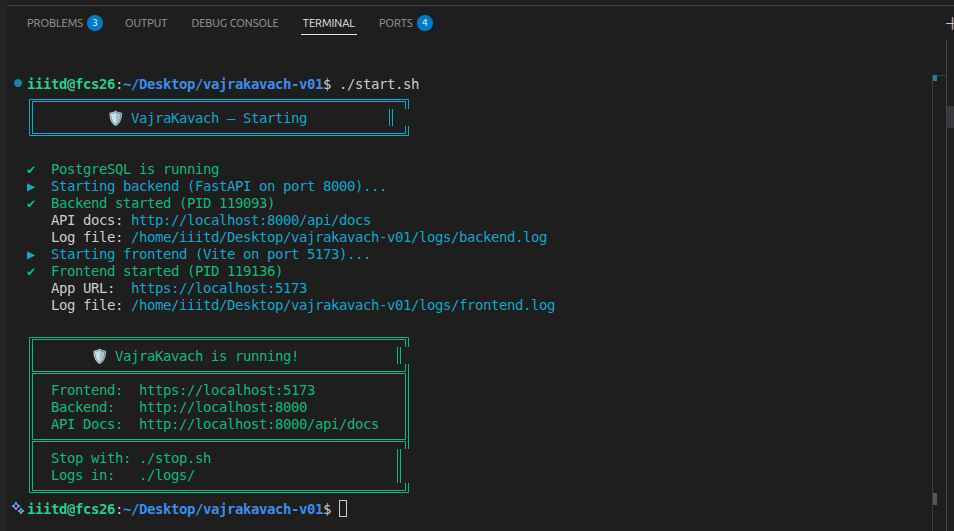
\includegraphics[width=0.95\textwidth]{screenshots/m1_https_terminal.png}
\caption{Terminal output showing the server starting with HTTPS on port 5173}
\end{figure}

\newpage

% ------ Section 3 ------
\section{Skeleton Application Deployment on VM}

The skeleton application was deployed on the IIITD VM with both backend and frontend running simultaneously.

\subsection{Project Structure}

\begin{lstlisting}
vajrakavach-v01/
  backend/
    app/
      main.py           # FastAPI application entry point
      config.py          # Environment configuration
      database.py        # Async SQLAlchemy engine + session
      dependencies.py    # Auth dependency injection
      models/            # SQLAlchemy ORM models
      routes/            # API route handlers
      services/          # Business logic services
    requirements.txt
    venv/
  frontend/
    src/
      pages/             # React page components
      components/        # Reusable UI components
      contexts/          # Auth context provider
      services/          # Axios API client
    vite.config.js
    package.json
  start.sh               # Starts both servers
  stop.sh                # Stops both servers
  logs/                   # Runtime log files
\end{lstlisting}

\subsection{Startup Process}

The \texttt{start.sh} script automates the full startup:
\begin{enumerate}
  \item Verifies PostgreSQL is running.
  \item Launches the FastAPI backend via Uvicorn on port 8000.
  \item Launches the Vite frontend dev server on port 5173 (HTTPS).
  \item Displays a summary with all URLs.
\end{enumerate}

\begin{lstlisting}
$ ./start.sh
  PostgreSQL is running
  Backend started (PID ...)
    API docs: http://localhost:8000/api/docs
  Frontend started (PID ...)
    App URL:  https://localhost:5173
\end{lstlisting}

\subsection{Screenshots}

\begin{figure}[H]
\centering

\includegraphics[width=0.95\textwidth]{screenshots/m1_terminal_start.png}
\caption{Terminal output of \texttt{start.sh} showing both servers launched successfully}
\end{figure}

\begin{figure}[H]
\centering

\includegraphics[width=0.95\textwidth]{screenshots/m1_skeleton_app.png}
\caption{Skeleton application landing page running on the VM}
\end{figure}

\begin{figure}[H]
\centering
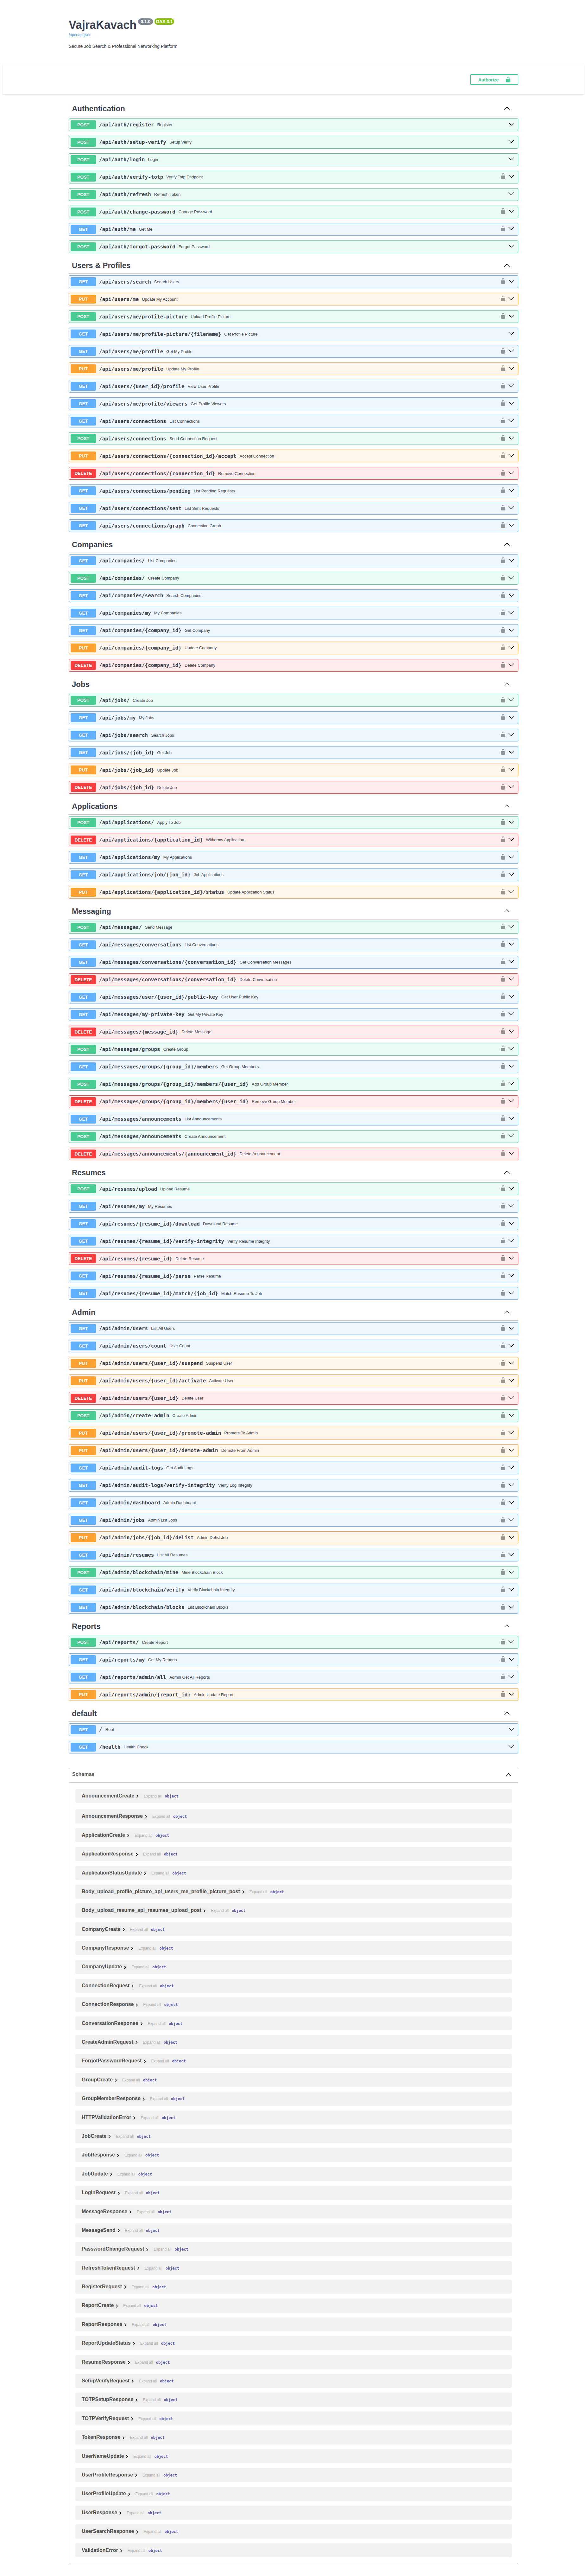
\includegraphics[width=0.95\textwidth]{screenshots/m1_api_docs.png}
\caption{FastAPI auto-generated Swagger UI at \texttt{/api/docs}}
\end{figure}

\newpage

% ------ Section 4 ------
\section{Summary}

For Milestone~1, we have:
\begin{enumerate}
  \item \textbf{Finalized the technology stack} --- FastAPI (Python) backend, React (Vite) frontend, PostgreSQL database, with Argon2id password hashing, JWT authentication, TOTP 2FA, Fernet and RSA encryption.
  \item \textbf{Configured HTTPS} --- Self-signed TLS certificates via \texttt{@vitejs/plugin-basic-ssl}, serving the frontend over \texttt{https://localhost:5173}.
  \item \textbf{Deployed a skeleton application} --- Both backend (port 8000) and frontend (port 5173) running on the IIITD VM with automated startup/shutdown scripts.
\end{enumerate}

The codebase is version-controlled on GitHub and ready for Milestone~2 feature development.

\vspace{1cm}
\noindent\textbf{Repository:} \url{https://github.com/yashkumarvaibhav/VajraKavach}

\end{document}
